% Chapter Template

\chapter{Ensayos y resultados} % Main chapter title

\label{Chapter4} % Change X to a consecutive number; for referencing this chapter elsewhere, use \ref{ChapterX}

%----------------------------------------------------------------------------------------
%	SECTION 1
%----------------------------------------------------------------------------------------
En este capítulo se detallan las pruebas realizadas durante el desarrollo del trabajo y finalmente se analizan los resultados obtenidos.
\section{Ensayos de funcionamiento y calibración del sensor de presión}
\label{sec:Ensayos de funcionamiento y calibración del sensor de presión}
Se llevó a cabo pruebas acerca del correcto funcionamiento y calibración del sensor de presión MPX5010DP. Para esto, como primera instancia se utilizó un osciloscopio como instrumento de medición de la señal derivada del sensor, una fuente de alimentación de 5 V para la energización del dispositivo y finalmente una manguera flexible de cristal cuyo diámetro externo es de 5 mm, 3 mm de diámetro interno y 300 mm de largo. Un extremo se conecta a una de las espigas del sensor y el otro se utiliza para introducir y evacuar agua mediante el uso de una jeringa. En la figura \ref{fig:Pruebas del sensor-Funcion patron.png} se puede apreciar la conexión del dispositivo trasnductor con la manguera flexible y con la herramienta de medición.    

\begin{figure}[htpb]
	\centering
	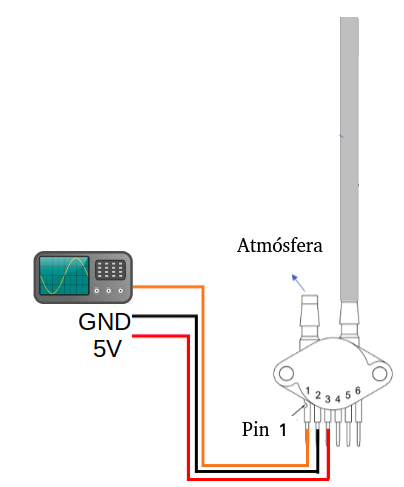
\includegraphics[scale=.50]{./Figures/PruebasDelSensor-FuncionPatron.png}
	\caption{Herramientas utilizadas para la verificación del funcionamiento del sensor y obtención de una función patrón. }
\label{fig:Pruebas del sensor-Funcion patron.png}
\end{figure}

La finalidad de este ensayo fue la adquisición datos para reconocer que el sensor presente un comportamiento lineal, Voltaje vs. Presión kPa, como lo especifica su respectiva hoja de datos. Para eso, a medida que se variaba	la altura de la columna de agua de la manguera se obtiene a la salida del sensor su correspondiente valor de voltaje. De esta forma, se logró generar una tabla con valores de Voltaje vs. Altura, que podremos corresponder con la presión, mediante la ecuación \ref{eq:presiónII}.
    
En la tabla \ref{tab:calibración del sensor-función patrón}, se puede apreciar que para cada valor de altura de columna de agua tiene asociado un valor de voltaje.  
\begin{table}[htpb]
	\centering
	\caption[Adquisición de datos para la calibración del sensor]{Adquisición de datos para la calibración del sensor.}
	\begin{tabular}{c c c}    
		\toprule
		\textbf{Número}     & \textbf{Altura[cm]} & \textbf{Voltios[V]} \\
		\midrule
		1  & 29,1          &  1.52 V \\		
		2  & 28,1          &  1,48 V \\
		3  & 25,25         &  1,4 V \\
		4  & 23,6          &  1,34 V \\
		5  & 21,9          & 1,26 V \\
		6  & 20,1          & 1,18 V \\
		7  & 17,82         & 1,06 V \\
		8  & 16,5          & 1,03 V \\
		9  & 15,4          & 0,96 V \\
		10 & 14,6          & 0,9 V \\
		11 & 12,7          & 0,84 V \\
		12 & 10,7          & 0,72 V \\
		13 & 8,3           & 0,66  V \\
		14 & 5,55          & 0,51 V \\
		15 & 3,5           & 0,46 V \\
		16 & 1,1           & 0,36 V \\
		17 & 0,7           & 0,3 V \\
		18 & 0,65          & 0,26 V \\
		19 & 0 cm          & 0,25 V \\
	
		\bottomrule
		\hline
	\end{tabular}
	\label{tab:calibración del sensor-función patrón}
\end{table}
A partir de los resultados conseguidos como se puede ver en la tabla \ref{tab:calibración del sensor-función patrón}, se pudo proyectar una gráfica que responde a una función lineal como se puede apreciar en la figura \ref{fig:Función patrón del sensor de presión calibrado: voltaje vs. altura}. 
Es importante notar en la gráfica de la figura \ref{fig:Función patrón del sensor de presión calibrado: voltaje vs. altura}, se encuentra presente un desplazamiento hacia arriba de la función de 0.250V respecto del eje de las abscisas, tal como lo especifica en la hoja de datos del sensor. Entonces para una altura de columna de agua de 0 cm el sensor está entregando a su salida 0.250V. 
Por lo tanto, luego de esta comprobación se concluyó que el sensor presentó un correcto desempeño.

\begin{figure}[H]
	\centering
	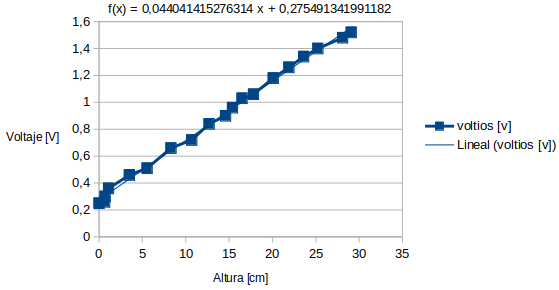
\includegraphics[scale=.75]{./Figures/FuncionPatron-Sensor-VoltajeVsAltura.png}
	\caption{Función patrón del sensor de presión calibrado: voltaje vs. altura.}
	\label{fig:Función patrón del sensor de presión calibrado: voltaje vs. altura}
	\end{figure}
%\vspace{2cm}	
	
\section{Calibración del sensor en el prototipo}
\label{sec:Calibración del sensor en el prototipo}
Una vez concluida la prueba de correcto funcionamiento del sensor y construido el prototipo se realizó un ensayo que consiste en la adquisición de datos del sistema completo mediante el empleo del firmware. Los datos proporcionados por dicho firmware fueron valores de presión, voltaje y altura del nivel de agua. Además, con el uso de una regla estándar como instrumento de medición, se obtuvo el nivel de agua real en el prototipo. Así, se logró realizar un ajuste, para la necesidad del trabajo en altura correspondiente a la columna de agua, utilizando una regresión lineal. La tabla \ref{tab:adquisición de datos del sistema I.}, muestra valores obtenidos en el ensayo realizado. Los mismos corresponden a un rango de altura comprendido entre el suelo del canal y el vértice del caudalímetro.

\begin{table}[htpb]
	\centering
	\caption[Adquisición de datos del sistema I]{Adquisición de datos del sistema I.}
	\begin{tabular}{c c c c c}    
		\toprule
		\textbf{Número}   & \textbf{Presión[Pa]}  & \textbf{Voltios[V]} & \textbf{Altura-Sistema[cm]} & \textbf{Altura-Real[cm]} \\
		\midrule
		1  & 0,065 & 0,229  & 0,66  & 1 \\
		2  & 0,1   & 0,245  & 1,03  & 1,5 \\
		3  & 0,136 & 0,261  & 1,39  & 2 \\
		4  & 0,179 & 0,281  & 1,83  & 2,6 \\
		5  & 0,229 & 0,303	& 2,35  & 3  \\
		6  & 0,272 & 0,323  & 2,79  & 3,5 \\
		7  & 0,315 & 0,342	& 3,23  & 4,1 \\
		8  & 0,351 & 0,358	& 3,6   & 4,5   \\
		9  & 0,401 & 0,381	& 4,11	& 5,1 \\
		10 & 0,444 & 0,4	& 4,55	& 5,5 \\
		11 & 0,487 & 0,419	& 4,99	& 6,1 \\
		12 & 0,523 & 0,435	& 5,36	& 6,5 \\
		13 & 0,566 & 0,455	& 5,8	& 7 \\
		14 & 0,616 & 0,477	& 6,31	& 7,5 \\
		15 & 0,667 & 0,5	& 6,82	& 8 \\
		16 & 0,703 & 0,516	& 7,19	& 8,5 \\
		17 & 0,753 & 0,539	& 7,7	& 9,05 \\
		18 & 0,81  & 0,565	& 8,29	& 9,55 \\
		19 & 0,846 & 0,581	& 8,66	& 10 \\
		20 & 0,896 & 0,603	& 9,17	& 10,5 \\
		21 & 0,939 & 0,623	& 9,61	& 11 \\
		22 & 0,996 & 0,648	& 10,2	& 11,5 \\
		23 & 1,039 & 0,668	& 10,64	& 12\\
		24 & 1,09  & 0,69	& 11,15	& 12,5 \\

	
		\bottomrule
		\hline
	\end{tabular}
	\label{tab:adquisición de datos del sistema I.}
\end{table}

De acuerdo con los valores expuestos en la tabla \ref{tab:adquisición de datos del sistema I.}, se puede reconocer que la altura entre el suelo del canal y el vértice del caudalímetro es de 12,5 cm. Entonces, si el nivel de altura de agua es menor o igual que dicho valor el caudal de agua es equivalente a cero, ya que no supera la altura del vértice de dicho caudalímetro.
En la tabla \ref{tab:adquisición de datos del sistema II.}, se aprecia que para una altura superior a los 12,5 cm, hay presencia de agua que fluye por la hendidura de la placa de aforo, por lo que se puede obtener valores de caudal de agua, litros/minuto vs altura h de columna de agua.
 
\begin{table}[htpb]
	\centering
	\caption[Adquisición de datos del sistema II]{Adquisición de datos del sistema II.}
	\begin{tabular}{c c c c c c}    
		\toprule
		\textbf{Número}   & \textbf{Presión[Pa]}  & \textbf{Vol.[V]} & \textbf{Alt.-Sistema[cm]} & \textbf{Alt.-Real[cm]} & \textbf{Caud.[l/m]} \\
		\midrule
		25  & 1     & 0,706  & 11,52  & 13   &  0,1\\
		26  & 1,19  & 0,735  & 12,18  & 13,6 &  0,3\\
		27  & 1,269 & 0,771  & 12,91  & 14,4 &  1 \\
		28  & 1,348 & 0,806  & 13,79  & 15,4 &  2,25 \\
		29  & 1,419 & 0,839	 & 14,53  & 16,1 &  3,74\\
		30  & 1,455 & 0,855  & 14,89  & 16,5 &  4,25\\
		31  & 1,47  & 0,861	 & 15,04  & 16,6 &  4,75\\
		32  & 1,491 & 0,871	 & 15,26  & 17,1 &  5,375\\
		
		\bottomrule
		\hline
	\end{tabular}
	\label{tab:adquisición de datos del sistema II.}
\end{table}

\vspace{1cm}

De la tabla \ref{tab:adquisición de datos del sistema II.}, se puede deducir que el valor máximo y mínimo de caudal obtenido es de 5,375 y 0,1 l/m respectivamente.
De la información obtenida a través de las mediciones que componen la tabla \ref{tab:adquisición de datos del sistema II.}, se extrajeron los valores correspondientes a las variables caudal y voltaje para construir la tabla \ref{tab:datos obtenidos para construir función polinómica de segundo grado.}.

\begin{table}[htpb]
	\centering
	\caption{Datos obtenidos para construir función polinómica de segundo grado.}
	\begin{tabular}{c c c }    
		\toprule
		\textbf{Número}   & \textbf{Voltios[V]} & \textbf{Caudal[l/m]}  \\
		\midrule
		1  & 0,706 & 0,1 \\
		2  & 0,771 & 1 \\
		3  & 0,806 & 2,25\\
		4  & 0,839 & 3,74 \\
		5  & 0,855 & 4,25  \\
		6  & 0,861 & 4,75 \\
		7  & 0,871 & 5,375 \\

		\bottomrule
		\hline
	\end{tabular}
	\label{tab:datos obtenidos para construir función polinómica de segundo grado.}
\end{table}
Estos datos se utilizaron para esbozar una gráfica y comprobar que responde a una función polinómica como la ecuación del modelo \ref{eq:caudal}. Seguidamente, en la figura \ref{fig:Función polinomica de segundo grado: caudal vs voltios}, se expone la gráfica obtenida y en la que se puede apreciar que manifiesta comportamientos de una función polinómica de segundo grado que involucra la variable caudal en función del voltaje.
 

\begin{figure}[H]
	\centering
	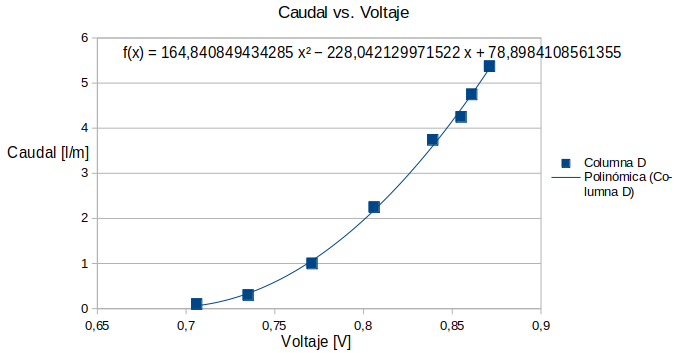
\includegraphics[scale=.60]{./Figures/FuncionPolinomicaCaudal-Voltaje.png}
	\caption{Función polinómica de segundo grado: caudal vs voltios.}
\label{fig:Función polinomica de segundo grado: caudal vs voltios}
\end{figure}



El diagrama correspondiente al prototipo se puede apreciar en la figura \ref{fig:Diagrama en bloque del prototipo}. En la imagen se observa que está compuesto por un depósito que suministra agua al banco de prueba. A su salida se encuentra una llave que durante los ensayos siempre está en el estado de apertura completa. Luego, se ubica la válvula de control con sus propios componentes que la conforman, el motor paso a paso, driver y fracción del firmware. Además se puede notar la presencia del algoritmo de control PI. Posterior a la válvula de control se puede dar con el canal que está construido por placas de madera impermeabilizadas para evitar filtraciones de agua. Finalmente se puede advertir el medidor de caudal constituido por el vertedero  con hendidura en V y el sensor de presión.
\begin{figure}[h]
	\centering
	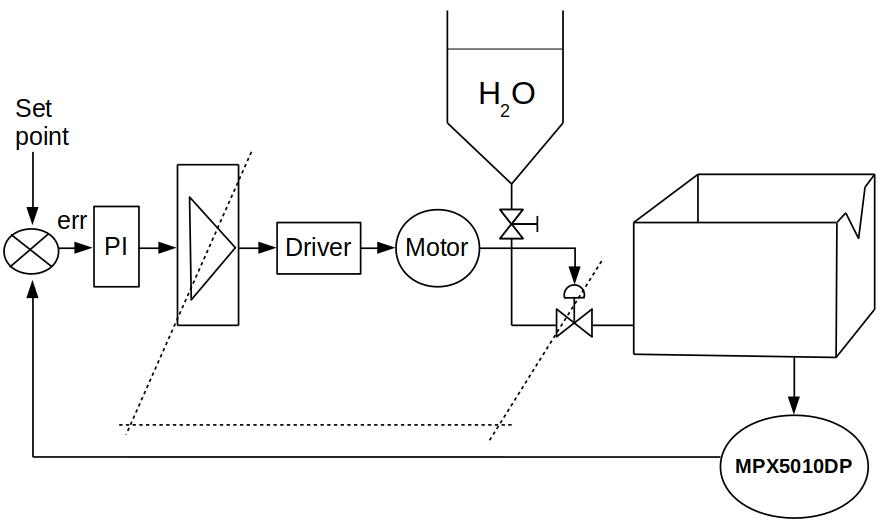
\includegraphics[scale=.60]{./Figures/Diagrama-prototipoII.png}
	\caption{Diagrama en bloque del prototipo.}
	\label{fig:Diagrama en bloque del prototipo}
\end{figure}	

\section{Resultados de las pruebas}
\label{sec:Resultados de las pruebas}
Al ser un entorno en el que se opera con agua, el tiempo mínimo para lograr el máximo caudal es de unos 120 segundos. Esto surgió de un ensayo realizado que consistió en abrir la válvula de 0\% al 100\% de manera manual e instantánea. Por esta razón, se determinó que el sistema posee un comportamiento lento por naturaleza. 
En la figura \ref{fig:Función de salida del sistema}, se puede apreciar que el sistema con lazo cerrado alcanza el estado de salida deseado. 

\begin{figure}[H]
	\centering
	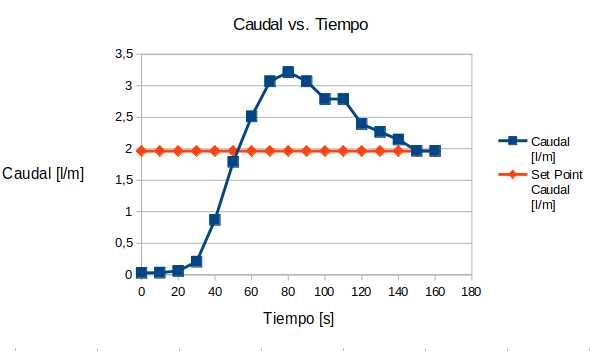
\includegraphics[scale=.80]{./Figures/FuncionDeSalidaDelSistema.png}
	\caption{Función de salida del sistema.}
	\label{fig:Función de salida del sistema}
\end{figure}

En este ensayo, se estableció un valor de consigna o set point del 35\% del valor máximo de caudal. En la función de salida, se puede notar que en el momento que existe un error y, más aún si es grande, el sistema tiende a minimizarlo.  
De esta forma, se puede observar que para llevar el caudal de 0\% al 35\% ocupa aproximadamente unos 150 segundos. Sin embargo, el sistema mostró un buen comportamiento durante las pruebas realizadas al establecer el caudal en 0\%, 25\%, 50\%,75\% y 100\% con idénticas respuestas esperadas de salida.  

%\begin{table}[h]
%	\centering
%	\caption[caption corto]{caption largo más descriptivo}
%	\begin{tabular}{l c c}    
%		\toprule
%		\textbf{Especie} 	 & \textbf{Tamaño} 		& \textbf{Valor}  \\
%		\midrule
%		Amphiprion Ocellaris & 10 cm 				& \$ 6.000 \\		
%		Hepatus Blue Tang	 & 15 cm				& \$ 7.000 \\
%		Zebrasoma Xanthurus	 & 12 cm				& \$ 6.800 \\
%		\bottomrule
%		\hline
%	\end{tabular}
%	\label{tab:peces}
%\end{table}

%La idea de esta sección es explicar cómo se hicieron los ensayos, qué resultados se obtuvieron y analizarlos.
